\documentclass[12pt, a4paper]{article}

\usepackage[utf8]{inputenc}

% Limit the page margin to only 1 inch.
\usepackage[margin=1in]{geometry}

%Imports biblatex package
\usepackage[
backend=biber,
style=alphabetic
]{biblatex}
\addbibresource{../math-342w.bib}

% Enables the `align' environment.
\usepackage{amsmath}
\allowdisplaybreaks
\usepackage{bm}
\usepackage{array}

% Provides useful environments, such as:
% - \begin{proof} ...\end{proof}
\usepackage{amsthm}
\newtheorem{proposition}{Proposition}
\theoremstyle{definition}
\newtheorem*{definition}{Definition}
\newtheorem{theorem}{Theorem}
\newtheorem{corollary}{Corollary}
\newtheorem*{example}{Example}
\newtheorem{algorithm}{Algorithm}

% Enables using \mathbb{}, for example \mathbb{N} for the set of natural numbers.
\usepackage{amssymb}

% Allows using letters in enumerate list environment. Use, for example:
%\begin{enumerate}[label=(\alph*)]
% ...
%\end{enumerate}
\usepackage[inline]{enumitem}

% Enable importing external graphic files and provides useful commands, like \graphicspath{}
\usepackage{graphicx}
% Images are located in a directory called "images" in the current directory.
\graphicspath{{./images/}}

% Make links look better by default.
% See: https://tex.stackexchange.com/questions/823/remove-ugly-borders-around-clickable-cross-references-and-hyperlinks
\usepackage[hidelinks]{hyperref}
\usepackage{xcolor}
\hypersetup{
	colorlinks,
	linkcolor={red!50!black},
	citecolor={blue!50!black},
	urlcolor={blue!80!black}
}

% Code Listings. Source:
% https://stackoverflow.com/questions/3175105/inserting-code-in-this-latex-document-with-indentation
\usepackage{listings}
\usepackage{color}
\usepackage[most]{tcolorbox}

\definecolor{dkgreen}{rgb}{0,0.6,0}
\definecolor{gray}{rgb}{0.5,0.5,0.5}
\definecolor{mauve}{rgb}{0.58,0,0.82}

\lstset{frame=tb,
	language=Java,
	aboveskip=3mm,
	belowskip=3mm,
	showstringspaces=false,
	columns=flexible,
	basicstyle={\small\ttfamily},
	numbers=none,
	numberstyle=\tiny\color{gray},
	keywordstyle=\color{blue},
	commentstyle=\color{dkgreen},
	stringstyle=\color{mauve},
	breaklines=true,
	breakatwhitespace=true,
	tabsize=3
}

\title{Lecture 21: MATH 342W: Introduction to Data Science and Machine Learning}
\author{Sergio E. Garcia Tapia\thanks{Based on lectures of Dr. Adam Kapelner at Queens College.
See also the \href{https://github.com/kapelner/QC_MATH_342W_Spring_2025}{course GitHub page}.}}
\date{April 29th, 2025 (last updated \today)}

\begin{document}
	\maketitle
	\section*{Bagging}
	Recall bagging, depicting in Figure~\ref{fig:bagging}.
	\begin{figure}
		\centering
		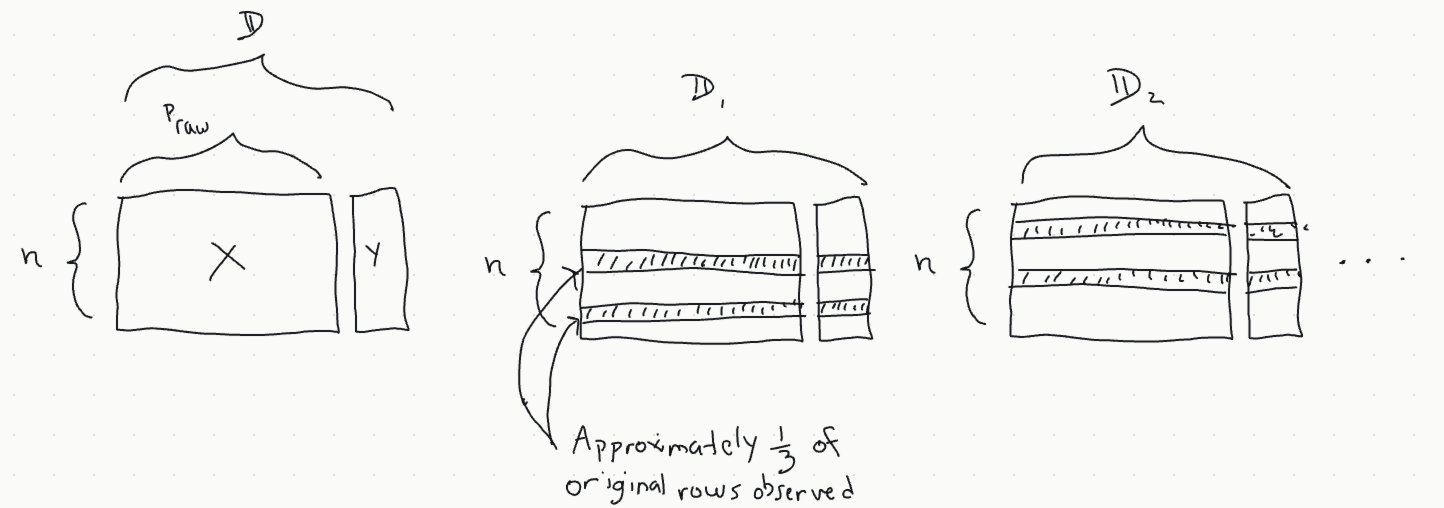
\includegraphics[width=0.9\textwidth]{bagging}
		\caption{Depiction of bagging. Each bootstraped sample contains about $\frac{2}{3}n$ of
		the original data.}
		\label{fig:bagging}
	\end{figure}
	How do we do validation for bagged models? Consider the first bootstrap sample
	$\mathbb{D}_1$, and the model we compute on it:
	\begin{align*}
		g_1 = \mathcal{A}(\mathbb{D}_1, \mathcal{H})
	\end{align*}
	Then $\mathbb{D}\setminus \mathbb{D}_1$ is out-of-sample for $g_1$. Thus,
	the metrics computed on $\mathbb{D}\setminus \mathbb{D}_1$ are honest.
	We can do the same for $g_2$ computed on bootstrap sample $\mathbb{D}_2$
	(likely different 1/3 of data missing than $\mathbb{D}_1$). We call this
	metric \textbf{out-of-bag (oob)}. If we do this $M$ times, we have $M$ models,
	each missing a slightly different 1/3 of the data (see Figure~\ref{fig:oob-data}).
	\begin{figure}
		\centering
		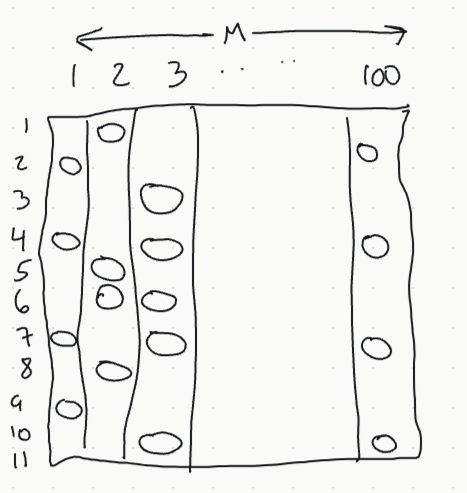
\includegraphics[width=0.3\textwidth]{out-of-bag-data-in-bootstrap-samples}
		\caption{Out-of-bag data in bootstrap samples. Each circle depicts
		which data point is missing from a given bootstrap sample.}
		\label{fig:oob-data}
	\end{figure}
	Thus for each unit,
	we can collect the models for which that unit is out-of-bag and use
	it them to compute an out-of-bag metric for $g_{avg}$:
	\begin{align*}
		g_{avg} := \frac{1}{M} \sum_{m=1}^{M}g_m
	\end{align*}
	\begin{tcolorbox}
		\begin{example}
			Given $M$ bootstrap models with index $\{1,2,\ldots,M\}$,
			suppose models $17, 37,88$ do not contain the observation
			$i=3$ (i.e., the data point $(\bm{x}_3,y_3)$ is out of bag
			for them). Then we can use models $g_{17}, g_{37}, g_{88}$
			to compute $\hat{y}_{17},\hat{y}_{37}, \hat{y}_{88}$ on
			$\bm{x}_3$. Thus, the out-of-bag value of $g_{avg}$ for
			observation $i=3$ is
			\begin{align*}
				\hat{y}_{oob, 3} = \text{Average}(\hat{y}_{17}, \hat{y}_{37}, \hat{y}_{88})
			\end{align*}
			We do this computation for all $i=1,2,\ldots,n$. In the sample
			above, the out-of-bag prediction was computed using 3 values.
			However, you will generally observe about $\frac{1}{3}M$ values
			included in the out-of-bag calculation.
		\end{example}
	\end{tcolorbox}
	Bagging is usually done with trees ($N_0 = 1$) because bias is low.
	\section*{Random Forests}
	Recall $\rho$ is the correlation between the trees. Thus, reducing $\rho$ means
	reducing decoupling between the trees. In 2001, Breiman brought the $\rho$ term in
	the Bias-Variance decomposition formula down even further. Breiman suggested that,
	instead of doing a full greedy search (as is done in regression trees), we can do
	the following:
	\begin{tcolorbox}
		\begin{algorithm}[Random Forest Algorithm]
			Use the bagged tree model with one change to the CART algorithm.
			Pick $m_{\text{try}} < p_{\text{raw}}$ and only search a random subset
			of $\{1,2,\ldots p_{\text{raw}}\}$ of size $m_{\text{try}}$ at each node.
			The ``reasonable" defaults for $m_{\text{try}}$ are
			$m_{\text{try}} = \lfloor p_{\text{raw}}/3\rfloor$ for regression,
			and $\lfloor \sqrt{p_{\text{raw}}}\rfloor$ for classification.
		\end{algorithm}
	\end{tcolorbox}
	Notice that the transition to random forests involves a change in the algorithm
	($\mathcal{A}$), not $\mathcal{H}$ or the features.
	\begin{tcolorbox}
		\begin{example}
			Let $p_{\text{raw}} = 10$, $m_{\text{try}} = 3$. For each root node,
			sample a subset of $m_{\text{try}} = 3$. For example, $\{x_3, x_7, x_9\}$,
			and do a greedy split based on those candidate splits only.
		\end{example}
	\end{tcolorbox}
	If $m_{\text{try}}$ is $p_{\text{raw}}$, then we have done nothing,
	since we would have the original regression tree algorithm. If $m_{\text{try}}$ is too
	low (say, $m_{\text{try}} = 1$), then you risk having a bias that is too large
	due to underfitting. In spite of the ``defaults" in place, you really should
	use model selection to optimize $m_{\text{try}}$, which is effectively a hyperparameter.
	
	Random forests contain two types of randomness: in the units and in the features.
	The term forest comes from the fact that we have multiple trees.
	\section*{R Demos}
	See \verb|QC_MATH_342W_Spring_2025/practice_lectures/lec21.Rmd|.
	\section*{Missingness}
	Suppose we have a data set $\mathbb{D}$ for which some units have missing features.
	That is, if we make a matrix $X$ containing the values of the features of all
	the units, then there are missing entries:
	
	In $R$, these would be \texttt{NA} values. Note that there is no missingness
	in the response $y$ (otherwise, it would not be in $\mathbb{D}$). If we have
	missing data, we cannot do this:
	\begin{align*}
		\bm{b} = (X^\top X)^{-1} X^\top \bm{y}
	\end{align*}
	For any of the algorithms $\mathcal{A}$ that we have discussed, we cannot have missing data.
	In the following lecture, we will discuss strategies for dealing with missing data in
	more detail.
	
	The simplest strategy is called \textbf{listwise deletion}, where we drop all subjects (rows)
	from $\mathbb{D}$ where there is at least one missing value. You shoudl only do this
	if $n$ is large and the number of missingness rows is ``very small". A down side of
	this is it incurs more estimation. There is another problem, to discussed next time.
\end{document}